\section{信号的分解}

这一章主要涉及傅里叶变换。假设我们有一个信号 $y = f(t)$,
我们希望能将其变成 $y' = F(\omega)$ 的形式。
我们可以考虑将 $f(t)$ 展开为
\begin{align*}
    f(t) = \sum_{n = -\infty}^{\infty} c_n\varphi_n(t)
\end{align*}
的形式,找出 $\varphi_n(t) = \mathe^{\mathi n\omega_i t}$ 中的常数 $w_i$。
这说明 $\varphi_n(t)$ 中含有关于 $w_i$ 的信息。
这样,统计 $f(t)$ 在频率域($\omega$)上的分布,我们就得到了 $F(\omega)$。

周期信号通常可以被表示为
\begin{align*}
    f(t) = \sum_{n = -\infty}^{\infty} f_0(t - nT),
\end{align*}
其中 $f_0(t)$ 是一个周期为 $T$ 的函数。

\subsection{信号的分解方法}

信号有多种方法可以进行分解:
\begin{itemize}
    \item 直流分量 + 交流分量
    \item 偶分量 + 奇分量
    \item 实部分量 + 虚部分量
    \item 脉冲分量
    \item 基于正交分量的分解
\end{itemize}

\begin{definition}[信号的直流/交流分解]
    设 $f(t)$ 为一个信号,定义其\bd{直流分量}为
    \begin{align*}
        f_{\text{AC}} = \lim_{T \to \infty}\frac{1}{T}\int_{T/2}^{-T/2}f(t)\D{t},
    \end{align*}
    其\bd{交流分量}为
    \begin{align*}
        f_{\text{AC}}(t) = f(t) - f_{\text{DC}}.
    \end{align*}
\end{definition}

\begin{definition}[信号的奇/偶分解]
    设 $f(t)$ 是一个信号,定义其\bd{奇分量}为
    \begin{align*}
        f_{\text{o}}(t) = \text{Od}[f(t)] = \frac{f(t) - f(-t)}{2},
    \end{align*}
    其\bd{偶分量}为
    \begin{align*}
        f_{\text{e}}(t) = \text{Ev}[f(t)] = \frac{f(t) + f(-t)}{2}.
    \end{align*}
\end{definition}

\begin{definition}[信号的实部/虚部分解]
    设 $f(t)$ 是一个信号,定义其\bd{实部分量}为
    \begin{align*}
        f_{\text{r}}(t) = \re[f(t)] = \frac{f(t) + f^*(t)}{2},
    \end{align*}
    其\bd{虚部分量}为
    \begin{align*}
        f_{\text{i}}(t) = \im[f(t)] = \frac{f(t) - f^*(t)}{2\mathi}.
    \end{align*}
\end{definition}

\begin{definition}[信号的脉冲分解]
    信号的\bd{脉冲分解}是指,信号可以近似地被表示为一组矩形脉冲的和的形式。
    设 $f(t)$ 是一个信号,定义其在 $t_1$ 处的矩形脉冲可以表示为如图 \ref{fig:rect-pulse-decomposition} 所示的函数:
    \begin{align*}
        f_{t_1}(t) = f(t_1)[u(t - t_1) - u(t - t_1 - \Delta t_1)],
    \end{align*}
    则 $f(t)$ 可以表示为
    \begin{align*}
        f(t) \approx \sum_{t_1 = -\infty}^{+\infty}f_{t_1}(t)
            = \sum_{t_1 = -\infty}^{+\infty}f(t_1)[u(t - t_1) - u(t - t_1 - \Delta t_1)].
    \end{align*}
    \begin{figure}[H]
        \centering
        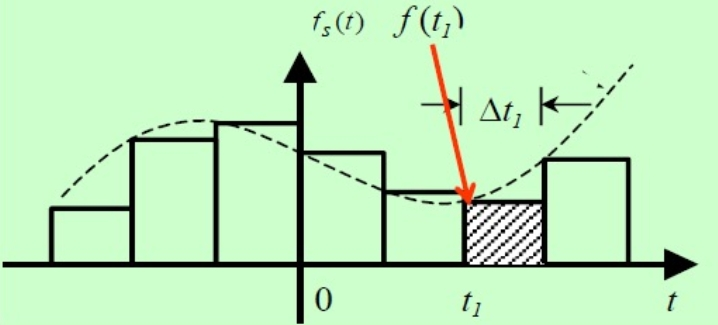
\includegraphics[width=0.5\textwidth]{chap2/img/rect-pulse-decomposition}
        \caption{$f(t)$ 的脉冲分解}
        \label{fig:rect-pulse-decomposition}
    \end{figure}
\end{definition}

\begin{note}
    信号的直流/交流分解、奇/偶分解、实部/虚部分解的结果是\bd{唯一}的,脉冲分解是结果是\bd{近似}的。
\end{note}

\subsection{函数的正交分解}

\subsubsection{标准正交函数集}

\begin{definition}[平方可积函数]
    令 $x(t)$ 为一实函数,若积分
    \begin{align*}
        \int_{-\infty}^{+\infty}x^2(t)\D{t}
    \end{align*}
    收敛,则称 $x(t)$ 为\bd{平方可积函数},记作 $x(t) \in L^2(\set{R})$。
    即,$L^2(\set{R})$ 表示所有平方可积函数组成的函数空间。
\end{definition}

\begin{definition}[内积]
    设 $f_1(t)$ 和 $f_2(t)$ 为两个函数,定义它们在区间 $[t_1, t_2]$ 上的\bd{内积}为
    \begin{align*}
        \ip{f_1}{f_2} = \int_{t_1}^{t_2}f_1(t)f_2^*(t)\D{t}.
    \end{align*}
\end{definition}

\begin{remark}
    回忆第 1 章中正交函数与正交函数集的定义,可以发现,$f_1(t)$ 和 $f_2(t)$ 在 $[t_1, t_2]$ 上正交,
    是指它们在 $[t_1, t_2]$ 上\bd{互不含有对方的分量}。函数 $f_1$ 和 $f_2$ 在 $[t_1, t_2]$ 上正交
    的充要条件是它们的内积为零。即,
    \begin{align*}
        \ip{f_1}{f_2} = 0.
    \end{align*}
\end{remark}

\begin{definition}[标准函数集]
    如果在区间 $[t_1, t_2]$ 上,函数集 $\{\varphi_i(t)\}$ 满足
    \begin{align*}
        \ip{\varphi_i}{\varphi_i} = \int_{t_1}^{t_2}\varphi_i(t)\varphi_i^*\D{t}
            = \int_{t_1}^{t_2}\|\varphi_i(t)\|^2\D{t} = 1,
    \end{align*}
    则称此函数集 $\{\varphi_i(t)\}$ 为\bd{标准函数集}。
\end{definition}

\begin{definition}[标准正交函数集]
    若正交函数集 $\{\varphi_i(t)\}$ 是一个标准函数集,则称之为\bd{标准正交函数集}。
\end{definition}

\subsubsection{函数的正交分解}

\begin{definition}[函数的正交分解]
    当函数 $f(t)$ 在 $[t_1, t_2]$ 区间具有连续的一阶导数和逐段连续的二阶导数时,
    $f(t)$ 可以用完备的正交函数集 $\{\varphi_i(t)\}$ 来表示,即
    \begin{align*}
        f(t) = \sum_{i = 1}^{+\infty}c_i\varphi_i(t),
    \end{align*}
    其中 $c_i$ 为常数,则称此表示为函数 $f(t)$ 的\bd{正交分解}。

    值得注意的是,$c_i$ 可以显式地表达为
    \begin{align*}
        c_i = \frac{\ip{f}{\varphi_i}}{\ip{\varphi_i}{\varphi_i}}
            = \frac{\ip{f}{\varphi_i}}{k_i}
            = \frac{1}{k_i}\int_{t_1}^{t_2}f(t)\varphi_i^*(t)\D{t},
    \end{align*}
    而 $k_i$ 为 $\varphi_i(t)$ 在区间 $[t_1, t_2]$ 上与自己的内积,即
    \begin{align*}
        k_i = \ip{\varphi_i}{\varphi_i} = \int_{t_1}^{t_2}\varphi_i(t)\varphi_i^*(t)\D{t}
        = \int_{t_1}^{t_2}\|\varphi_i(t)\|^2\D{t}.
    \end{align*}
\end{definition}

\begin{theorem}[帕斯瓦尔定理]
    用一个正交函数集来准确地表示一个信号时,这信号的能量等于相应的正交函数各分量的能量之和。
    即,设 $f(t)$ 为一个信号,将用正交函数集 $\{\varphi_i(t)\}$ 来表示,$c_i, k_i$ 定义如上,
    则有
    \begin{align*}
        \int_{t_1}^{t_2}\|f(t)\|^2\D{t} = \sum_{i = 1}^{+\infty}\|c_i\|^2k_i.
    \end{align*}
    这被称为\bd{帕斯瓦尔(Parseval)定理}。
\end{theorem}

\begin{proof}
    由于 $\{\varphi_i(t)\}$ 是一个正交函数集,故有
    \begin{align*}
        \ip{\varphi_i}{\varphi_j} = \begin{cases}
            1, & i = j, \\
            0, & i \neq j.
        \end{cases}
    \end{align*}
    而 $f(t)$ 的正交分解为 $f(t) = \sum_{i = 1}^{+\infty}c_i\varphi_i(t)$,故有
    \begin{align*}
        \int_{t_1}^{t_2}\|f(t)\|^2\D{t} & = \int_{t_1}^{t_2}\left\|\sum_{i = 1}^{+\infty}c_i\varphi_i(t)\right\|^2\D{t} \\
        & = \int_{t_1}^{t_2}\sum_{i = 1}^{+\infty}\|c_i\varphi_i(t)\|^2\D{t}
            + \sum_{i, j \ge 1, i \neq j}\|c_ic_j^*\ip{\varphi_i}{\varphi_j}\| \\
        & = \int_{t_1}^{t_2}\sum_{i = 1}^{+\infty}\|c_i\|^2\cdot \|\varphi_i(t)\|^2\D{t} + 0 \\
        & = \sum_{i = 1}^{+\infty}\|c_i\|^2k_i.
    \end{align*}
\end{proof}

\begin{note}
    在推导的过程中,对于内积运算,别忘了\bd{取共轭}。例如上述证明中的 $c_j^*$。
\end{note}

\subsection{信号的正交变换}

\subsubsection{信号的级数展开}

\begin{definition}[信号的级数展开]
    考虑使用一组函数 $\{\varphi_i(t)\}$,将信号 $x(t) \in L^2(\set{R})$ 展开成级数,即
    \begin{align*}
        x(t) = \sum_{i = -\infty}^{+\infty}c_i\varphi_i(t),
    \end{align*}
    这一形式称为信号 $x(t)$ 的\bd{级数展开}。

    通常,展开系数 $c_i$ 使用信号 $x(t)$ 的某种积分形式来确定。这一积分公式(即求展开系数的公式)
    称之为\bd{信号变换}。
\end{definition}

\subsubsection{函数的正交变换}

\begin{definition}[函数的正交变换]
    若信号级数展开的基函数 $\{\varphi_i(t)\}$ 为标准完备正交函数集,则积分变换
    \begin{align*}
        c_i = \int_{t_1}^{t_2}x(t)\varphi_i^*(t)\D{t}
    \end{align*}
    称为信号 $x(t)$ 的\bd{正交变换},亦称为 \bd{Karhunen-Loève 变换}。
\end{definition}

\begin{note}
    如果信号为符合狄义赫利(Dirichlet)条件的周期函数,则正交分解的系数 $c_i$ 的形式会很漂亮。
\end{note}

